%%%%%%%%%%%%%%%%%%%%%%%%%%%%%%%%%%%%%%%%%
% Short Sectioned Assignment
% LaTeX Template
% Version 1.0 (5/5/12)
%
% This template has been downloaded from:
% http://www.LaTeXTemplates.com
%
% Original author:
% Frits Wenneker (http://www.howtotex.com)
%
% License:
% CC BY-NC-SA 3.0 (http://creativecommons.org/licenses/by-nc-sa/3.0/)
%
%%%%%%%%%%%%%%%%%%%%%%%%%%%%%%%%%%%%%%%%%

%----------------------------------------------------------------------------------------
%	PACKAGES AND OTHER DOCUMENT CONFIGURATIONS
%----------------------------------------------------------------------------------------

\documentclass[paper=a4, fontsize=11pt]{scrartcl} % A4 paper and 11pt font size

%\usepackage[T1]{fontenc} % Use 8-bit encoding that has 256 glyphs
\usepackage[utf8]{inputenc}
\usepackage{fourier} % Use the Adobe Utopia font for the document - comment this line to return to the LaTeX default
\usepackage[portuguese]{babel} % English language/hyphenation
\usepackage{amsmath,amsfonts,amsthm} % Math packages

\usepackage{lipsum} % Used for inserting dummy 'Lorem ipsum' text into the template

\usepackage{sectsty} % Allows customizing section commands
\allsectionsfont{\centering \normalfont\scshape} % Make all sections centered, the default font and small caps

\usepackage{fancyhdr} % Custom headers and footers

\usepackage{url}
\usepackage{graphicx}
\usepackage{caption}
\usepackage{subcaption} 
\usepackage{multirow}

\pagestyle{fancyplain} % Makes all pages in the document conform to the custom headers and footers
\fancyhead{} % No page header - if you want one, create it in the same way as the footers below
\fancyfoot[L]{} % Empty left footer
\fancyfoot[C]{} % Empty center footer
\fancyfoot[R]{\thepage} % Page numbering for right footer
\renewcommand{\headrulewidth}{0pt} % Remove header underlines
\renewcommand{\footrulewidth}{0pt} % Remove footer underlines
\setlength{\headheight}{13.6pt} % Customize the height of the header

\numberwithin{equation}{section} % Number equations within sections (i.e. 1.1, 1.2, 2.1, 2.2 instead of 1, 2, 3, 4)
\numberwithin{figure}{section} % Number figures within sections (i.e. 1.1, 1.2, 2.1, 2.2 instead of 1, 2, 3, 4)
\numberwithin{table}{section} % Number tables within sections (i.e. 1.1, 1.2, 2.1, 2.2 instead of 1, 2, 3, 4)

\setlength\parindent{0pt} % Removes all indentation from paragraphs - comment this line for an assignment with lots of text

%----------------------------------------------------------------------------------------
%	TITLE SECTION
%----------------------------------------------------------------------------------------

\newcommand{\horrule}[1]{\rule{\linewidth}{#1}} % Create horizontal rule command with 1 argument of height

\title{	
\normalfont \normalsize 
\textsc{Universidade Federal do Paraná} \\ [25pt] % Your university, school and/or department name(s)
\horrule{0.5pt} \\[0.4cm] % Thin top horizontal rule
\huge Reconhecimento de Padrões \\
\large Trabalho final  % The assignment title
\horrule{2pt} \\[0.5cm] % Thick bottom horizontal rule
}

\author{Gian Maurício Fritsche} % Your name

\date{\normalsize\today} % Today's date or a custom date

\begin{document}

\maketitle % Print the title

%----------------------------------------------------------------------------------------
%	PROBLEM 1
%----------------------------------------------------------------------------------------

\section{Descrição do trabalho}

Para a realização deste trabalho foi utilizada a base de imagens SIMPSONS\footnote{\url{http://www.inf.ufpr.br/lesoliveira/padroes/simpsons.zip}}.
O objetivo é construir um sistema de reconhecimento de padrões que discrimine as cinco classes (representando os cinco personagens principais: Bart, Homer, Lisa, Maggie e Marge).

\begin{figure}
    \centering
    \begin{subfigure}[b]{0.15\textwidth}
        
\includegraphics[width=\textwidth]{bart001}
        \caption{Bart}
        \label{fig:bart}
    \end{subfigure}
    ~ %add desired spacing between images, e. g. ~, \quad, \qquad, \hfill etc. 
      %(or a blank line to force the subfigure onto a new line)
    \begin{subfigure}[b]{0.15\textwidth}
        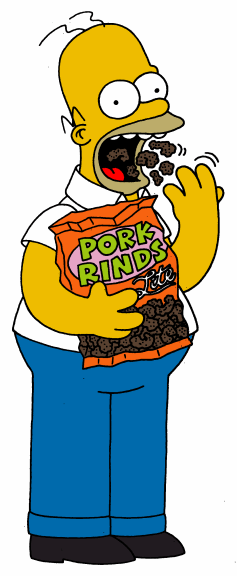
\includegraphics[width=\textwidth]{homer001}
        \caption{Homer}
        \label{fig:homer}
    \end{subfigure}
    ~ %add desired spacing between images, e. g. ~, \quad, \qquad, \hfill etc. 
    %(or a blank line to force the subfigure onto a new line)
    \begin{subfigure}[b]{0.15\textwidth}
        
\includegraphics[width=\textwidth]{lisa001}
        \caption{Lisa}
        \label{fig:lisa}
    \end{subfigure}
    ~ %add desired spacing between images, e. g. ~, \quad, \qquad, \hfill etc. 
    %(or a blank line to force the subfigure onto a new line)
    \begin{subfigure}[b]{0.15\textwidth}
        
\includegraphics[width=\textwidth]{maggie001}
        \caption{Maggie}
        \label{fig:maggie}
    \end{subfigure}
    ~ %add desired spacing between images, e. g. ~, \quad, \qquad, \hfill etc. 
    %(or a blank line to force the subfigure onto a new line)
    \begin{subfigure}[b]{0.15\textwidth}
        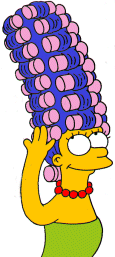
\includegraphics[width=\textwidth]{marge001}
        \caption{Marge}
        \label{fig:marge}
    \end{subfigure}
    \caption{Exemplos de imagens}\label{fig:exemplos}
\end{figure}

Na Figura~\ref{fig:exemplos} são apresentados exemplos de imagens para cada uma das cinco classes.
Foram utilizados três métodos para extração de características: Histograma de cor, Momentos de Hu e Histograma da orientação dos gradientes {\it Histogram of oriented gradients} (HOG).
Inicialmente toda imagem recebida pelo módulo de extração é redimensionada para $150 \times 150$, em seguida é enviada para o método de extração de características selecionado.

\subsection{Extração de características}

Para o histograma de cor, cada canal (cor de 0 à 255) foi dividida em quatro partes (bins) e calculado quantos pixels se encaixam em cada parte (para cada cor). 
Retornando assim um vetor de características com 64 posições.
A quantidade de divisões (bins) é um parâmetro do método, porém apenas o valor quatro foi avaliado.
Outro método de extração de características utilizado foi o Momentos de Hu, que são invariantes a translação, rotação e escala.
Para sua utilização a imagem foi convertida para tons de cinza. Este método retorna um vetor de sete características (os sete momentos de Hu).
É sugerido que este método seja utilizado após a segmentação da imagem, porém esta etapa não foi realizada.
O terceiro método de extração de características utilizado foi o HOG, que utiliza os gradientes da imagem para capturar contornos, silhuetas e algumas informações de textura.

\subsection{Classificação}

Para a classificação das imagens, inicialmente os vetores de característica são normalizados.
Em seguida é aplicado um dos três classificadores implementados: {\it Linear Discriminant Analysis} (LDA), {\it K-th Nearest Neighbor} (KNN) e {\it Support Vector Machine } (SVM).
O método KNN, apresenta dois parâmetros, o número de vizinhos ($k$) e a métrica de distância.
Os valores utilizados foram $k=5$ e distância euclidiana. Não foram avaliados outros valores.
Para o SVM o modelo foi aprendido por meio de {\it GridSearch}.

\subsection {Fusão}

Para a fusão foram construídas duas lista, uma com os métodos de extração de características ({\it features}) e outra com os classificadores ({\it clasifiers}).
Então para cada combinação $[feature, classifier]$ é construído e treinado um classificador.
Em seguida os exemplos de teste são classificados utilizando todos os classificadores construídos.
Para a fusão da saída dos classificadores foram implementados cinco métodos: soma, mínimo, máximo, produto e {\it borda count}.
Os quatro primeiros utilizam as probabilidades retornadas por cada classificador, 
enquanto para o {\it borda count} foi calculado os rankings (a partir das probabilidades).

\section {Análise da classificação}
% Please add the following required packages to your document preamble:
% \usepackage{multirow}
\begin{table}[!htb]
\centering
\caption{Matrizes de confusão para os classificadores utilizando Histograma de Cor}
\label{tbl:colorhistogram}
\begin{tabular}{l|l|l|l|l|l|l}
\hline
\multicolumn{7}{l}{\textbf{Classifier: svm}}                                                \\ \hline
\multicolumn{7}{l}{\textbf{Score 62.11\%}}                                                  \\ \hline
          & bart      & homer     & lisa      & maggie    & marge          & score            \\ \hline
bart      & 27        & 7         & 1         & 0         & 0              & 77.14\%          \\ \hline
homer     & 5         & 15        & 3         & 1         & 1              & 60.00\%          \\ \hline
lisa      & 4         & 3         & 6         & 0         & 0              & 46.15\%          \\ \hline
maggie    & 1         & 3         & 0         & 8         & 0              & 66.67\%          \\ \hline
marge     & 5         & 1         & 1         & 0         & 3              & 30.00\%          \\ \hline
          &           &           & \textbf{} & \textbf{} & \textbf{media} & \textbf{55.99\%} \\ \hline
\multicolumn{7}{l}{\textbf{Classifier: lda}}                                                \\ \hline
\multicolumn{7}{l}{\textbf{Score 68.42\%}}                                                  \\ \hline
          & bart      & homer     & lisa      & maggie    & marge          & score            \\ \hline
bart      & 30        & 4         & 1         & 0         & 0              & 85.71\%          \\ \hline
homer     & 2         & 16        & 6         & 0         & 1              & 64.00\%          \\ \hline
lisa      & 2         & 3         & 8         & 0         & 0              & 61.54\%          \\ \hline
maggie    & 2         & 2         & 0         & 8         & 0              & 66.67\%          \\ \hline
marge     & 3         & 1         & 3         & 0         & 3              & 30.00\%          \\ \hline
          &           &           &           &           & \textbf{media} & \textbf{61.58\%} \\ \hline
\multicolumn{7}{l}{\textbf{Classifier: knn}}                                                \\ \hline
\multicolumn{7}{l}{\textbf{Score 65.26\%}}                                                  \\ \hline
          & bart      & homer     & lisa      & maggie    & marge          & score            \\ \hline
bart      & 32        & 2         & 1         & 0         & 0              & 91.43\%          \\ \hline
homer     & 7         & 12        & 5         & 1         & 0              & 48.00\%          \\ \hline
lisa      & 3         & 1         & 8         & 1         & 0              & 61.54\%          \\ \hline
maggie    & 4         & 1         & 0         & 7         & 0              & 58.33\%          \\ \hline
marge     & 7         & 0         & 0         & 0         & 3              & 30.00\%          \\ \hline
          &           &           &           & \textbf{} & \textbf{media} & \textbf{57.86\%} \\ \hline
\end{tabular}
\end{table}

\begin{table}[!htb]
\centering
\caption{Matrizes de confusão para os classificadores utilizando Histograma de orientação dos gradientes}
\label{tbl:hog}
\begin{tabular}{l|l|l|l|l|l|l} \hline
\multicolumn{7}{l}{\textbf{Classifier: svm}}                                                \\ \hline
\multicolumn{7}{l}{\textbf{Score 43.16\%}}                                                  \\ \hline
          & bart      & homer     & lisa      & maggie    & marge          & score            \\ \hline
bart      & 26        & 9         & 0         & 0         & 0              & 74.29\%          \\ \hline
homer     & 14        & 9         & 1         & 0         & 1              & 36.00\%          \\ \hline
lisa      & 5         & 5         & 3         & 0         & 0              & 23.08\%          \\ \hline
maggie    & 3         & 5         & 1         & 2         & 1              & 16.67\%          \\ \hline
marge     & 5         & 3         & 1         & 0         & 1              & 10.00\%          \\ \hline
          &           &           &           &           & \textbf{media} & \textbf{32.01\%} \\ \hline
\multicolumn{7}{l}{\textbf{Classifier: lda}}                                                \\ \hline
\multicolumn{7}{l}{\textbf{Score 43.16\%}}                                                  \\ \hline
          & bart      & homer     & lisa      & maggie    & marge          & score            \\ \hline
bart      & 26        & 6         & 2         & 1         & 0              & 74.29\%          \\ \hline
homer     & 11        & 9         & 0         & 2         & 3              & 36.00\%          \\ \hline
lisa      & 9         & 3         & 1         & 0         & 0              & 7.69\%           \\ \hline
maggie    & 6         & 2         & 0         & 4         & 0              & 33.33\%          \\ \hline
marge     & 6         & 2         & 1         & 0         & 1              & 10.00\%          \\ \hline
          &           &           &           &           & \textbf{media} & \textbf{32.26\%} \\ \hline
\multicolumn{7}{l}{\textbf{Classifier: knn}}                                                \\ \hline
\multicolumn{7}{l}{\textbf{Score 49.47\%}}                                                  \\ \hline
          & bart      & homer     & lisa      & maggie    & marge          & score            \\ \hline
bart      & 32        & 3         & 0         & 0         & 0              & 91.43\%          \\ \hline
homer     & 11        & 14        & 0         & 0         & 0              & 56.00\%          \\ \hline
lisa      & 8         & 4         & 1         & 0         & 0              & 7.69\%           \\ \hline
maggie    & 9         & 3         & 0         & 0         & 0              & 0.00\%           \\ \hline
marge     & 7         & 3         & 0         & 0         & 0              & 0.00\%           \\ \hline
          &           &           &           &           & \textbf{media} & \textbf{31.02\%} \\ \hline
\multicolumn{7}{l}{\multirow{2}{*}{}}                                                       \\
\end{tabular}
\end{table}

\begin{table}[!htb]
\centering
\caption{Matrizes de confusão para os classificadores utilizando Momentos de Hu}
\label{tbl:hog}
\begin{tabular}{l|l|l|l|l|l|l} \hline
\multicolumn{7}{l}{\textbf{Classifier: svm}}                                                \\ \hline
\multicolumn{7}{l}{\textbf{Score 44.21\%}}                                                  \\ \hline
          & bart      & homer     & lisa      & maggie    & marge          & score            \\ \hline
bart      & 28        & 7         & 0         & 0         & 0              & 80.00\%          \\ \hline
homer     & 14        & 9         & 0         & 2         & 0              & 36.00\%          \\ \hline
lisa      & 11        & 2         & 0         & 0         & 0              & 0.00\%           \\ \hline
maggie    & 8         & 3         & 0         & 0         & 1              & 0.00\%           \\ \hline
marge     & 3         & 2         & 0         & 0         & 5              & 50.00\%          \\ \hline
\textbf{} & \textbf{} & \textbf{} & \textbf{} & \textbf{} & \textbf{media} & \textbf{33.20\%} \\ \hline
\multicolumn{7}{l}{\textbf{Classifier: lda}}                                                \\ \hline
\multicolumn{7}{l}{\textbf{Score 41.05\%}}                                                  \\ \hline
          & bart      & homer     & lisa      & maggie    & marge          & score            \\ \hline
bart      & 25        & 6         & 0         & 1         & 3              & 71.43\%          \\ \hline
homer     & 15        & 7         & 0         & 3         & 0              & 28.00\%          \\ \hline
lisa      & 11        & 1         & 0         & 0         & 1              & 0.00\%           \\ \hline
maggie    & 8         & 1         & 0         & 1         & 2              & 8.33\%           \\ \hline
marge     & 3         & 1         & 0         & 0         & 6              & 60.00\%          \\ \hline
\textbf{} & \textbf{} & \textbf{} & \textbf{} & \textbf{} & \textbf{media} & \textbf{33.55\%} \\ \hline
\multicolumn{7}{l}{\textbf{Classifier: knn}}                                                \\ \hline
\multicolumn{7}{l}{\textbf{Score 37.89\%}}                                                  \\ \hline
          & bart      & homer     & lisa      & maggie    & marge          & score            \\ \hline
bart      & 20        & 6         & 6         & 1         & 2              & 57.14\%          \\ \hline
homer     & 10        & 8         & 3         & 3         & 1              & 32.00\%          \\ \hline
lisa      & 10        & 0         & 0         & 2         & 1              & 0.00\%           \\ \hline
maggie    & 4         & 2         & 1         & 3         & 2              & 25.00\%          \\ \hline
marge     & 2         & 1         & 1         & 1         & 5              & 50.00\%          \\ \hline
\textbf{} & \textbf{} & \textbf{} & \textbf{} & \textbf{} & \textbf{media} & \textbf{32.83\%} \\ \hline
\end{tabular}
\end{table}

\begin{table}[]
\centering
\caption{Fusão dos nove métodos de classificação instanciados}
\label{tbl:fusionall}
\begin{tabular}{l|l|l|l|l|l|l}
\hline
\multicolumn{7}{l}{\textbf{borda}}                                                          \\ \hline
\multicolumn{7}{l}{\textbf{Score: 53.68\%}}                                                 \\ \hline
          & bart      & homer     & lisa      & maggie    & marge          & score            \\ \hline
bart      & 34        & 1         & 0         & 0         & 0              & 97.14\%          \\ \hline
homer     & 13        & 12        & 0         & 0         & 0              & 48.00\%          \\ \hline
lisa      & 11        & 1         & 1         & 0         & 0              & 7.69\%           \\ \hline
maggie    & 7         & 3         & 0         & 2         & 0              & 16.67\%          \\ \hline
marge     & 8         & 0         & 0         & 0         & 2              & 20.00\%          \\ \hline
\textbf{} & \textbf{} & \textbf{} & \textbf{} & \textbf{} & \textbf{media} & \textbf{37.90\%} \\ \hline
\multicolumn{7}{l}{\textbf{sum}}                                                            \\ \hline
\multicolumn{7}{l}{\textbf{Score: 67.37\%}}                                                 \\ \hline
          & bart      & homer     & lisa      & maggie    & marge          & score            \\ \hline
bart      & 33        & 2         & 0         & 0         & 0              & 94.29\%          \\ \hline
homer     & 7         & 17        & 1         & 0         & 0              & 68.00\%          \\ \hline
lisa      & 8         & 3         & 2         & 0         & 0              & 15.38\%          \\ \hline
maggie    & 2         & 2         & 0         & 8         & 0              & 66.67\%          \\ \hline
marge     & 4         & 1         & 1         & 0         & 4              & 40.00\%          \\ \hline
\textbf{} & \textbf{} & \textbf{} & \textbf{} & \textbf{} & \textbf{media} & \textbf{56.87\%} \\ \hline
\multicolumn{7}{l}{\textbf{max}}                                                            \\ \hline
\multicolumn{7}{l}{\textbf{Score: 63.16\%}}                                                 \\ \hline
          & bart      & homer     & lisa      & maggie    & marge          & score            \\ \hline
bart      & 29        & 3         & 2         & 1         & 0              & 82.86\%          \\ \hline
homer     & 6         & 12        & 6         & 0         & 1              & 48.00\%          \\ \hline
lisa      & 3         & 3         & 7         & 0         & 0              & 53.85\%          \\ \hline
maggie    & 2         & 2         & 0         & 8         & 0              & 66.67\%          \\ \hline
marge     & 3         & 1         & 2         & 0         & 4              & 40.00\%          \\ \hline
\textbf{} & \textbf{} & \textbf{} & \textbf{} & \textbf{} & \textbf{media} & \textbf{58.27\%} \\ \hline
\multicolumn{7}{l}{\textbf{min}}                                                            \\ \hline
\multicolumn{7}{l}{\textbf{Score: 47.37\%}}                                                 \\ \hline
          & bart      & homer     & lisa      & maggie    & marge          & score            \\ \hline
bart      & 31        & 3         & 0         & 1         & 0              & 88.57\%          \\ \hline
homer     & 14        & 11        & 0         & 0         & 0              & 44.00\%          \\ \hline
lisa      & 12        & 1         & 0         & 0         & 0              & 0.00\%           \\ \hline
maggie    & 7         & 1         & 1         & 3         & 0              & 25.00\%          \\ \hline
marge     & 9         & 1         & 0         & 0         & 0              & 0.00\%           \\ \hline
\textbf{} & \textbf{} & \textbf{} & \textbf{} & \textbf{} & \textbf{media} & \textbf{31.51\%} \\ \hline
\multicolumn{7}{l}{\textbf{product}}                                                        \\ \hline
\multicolumn{7}{l}{\textbf{Score: 47.37\%}}                                                 \\ \hline
          & bart      & homer     & lisa      & maggie    & marge          & score            \\ \hline
bart      & 32        & 3         & 0         & 0         & 0              & 91.43\%          \\ \hline
homer     & 15        & 10        & 0         & 0         & 0              & 40.00\%          \\ \hline
lisa      & 12        & 1         & 0         & 0         & 0              & 0.00\%           \\ \hline
maggie    & 7         & 1         & 1         & 3         & 0              & 25.00\%          \\ \hline
marge     & 9         & 1         & 0         & 0         & 0              & 0.00\%           \\ \hline
\textbf{} & \textbf{} & \textbf{} & \textbf{} & \textbf{} & \textbf{media} & \textbf{31.29\%} \\ \hline
\end{tabular}
\end{table}

\end{document}